\chapter{Obiekt regulacji}
\label{cha:ch2_obiekt_regulacji}

Obiektem poddawanym regulacji był system typu kulka na belce, który został zbudowany od podstaw na potrzeby tej pracy.

%%%%%%%%
\section{Obiekty typu kulka na belce}

Na system tego typu składają się długa, umieszczona horyzontalnie belka i silnik lub serwomechanizm, który umożliwia wychylanie się belki.
Po belce swobodnie porusza się kulka.

Podstawowym zadaniem regulacji w systemie tego typu jest stabilizacja położenia kulki w wybranym punkcie.
Charakterystyczną cechą tego systemu jest prostota konstrukcji oraz niestabilność przy braku aktywnej regulacji.

Obiekty tego typu są często wykorzystywane w dydaktyce teorii sterowania. Składają się na to poniższe powody:

\begin{itemize}
	\item prostota budowy,
	\item możliwość zastosowania różnych czujników położenia kulki,
	\item możliwość zastosowania różnych silników i mechanizmów przeniesienia napędu.
\end{itemize}

Uproszczony schemat systemu kulka i belka przedstawiony został poniżej:

\begin{figure}[H]
	\centering
	\includesvg[width=0.7\textwidth,svgpath=./graphics/]{kulka_belka_schemat_uproszczony}
	\caption{Uproszczony schemat systemu typu kulka i belka.}
	\label{fig:kulka_belka_schemat_uproszczony}
\end{figure}

% TODO: dodać źródła
Prostota konstrukcji i inherentna niestabilność sprawiły, że powstało wiele implementacji tego systemu [1][2][3][4], również komercyjne, jak na przykład produkt firmy Quanser:

\begin{figure}[H]
	\centering
	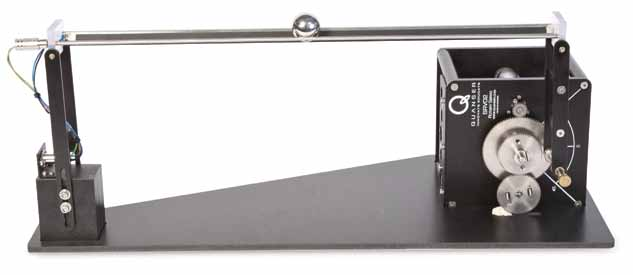
\includegraphics[width=0.5\textwidth]{quanser_ball_beam}
	\caption{Zdjęcie produktu \textit{Ball and Beam} firmy Quanser.}
	\label{fig:quanser_ball_beam}
% TODO: dodać źródło
\end{figure}

%%%%%%%%
\section{Projekt mechaniczny}

Przed przystąpieniem do budowy obiektu, zaprojektowano wstępny kształt w programie \textsc{CAD} \texttt{SketchUp Make} (\cref{fig:cad_render_1}). Wyszczególniono na nim:

\begin{itemize}
	\item prostokątną podstawę,
	\item słupy podtrzymujące belkę,
	\item usztywniający łącznik między słupami,
	\item oś obrotu (wał) umieszczony w połowie długości belki,
	\item przekrój belki.
\end{itemize}

\begin{figure}[H]
	\centering
	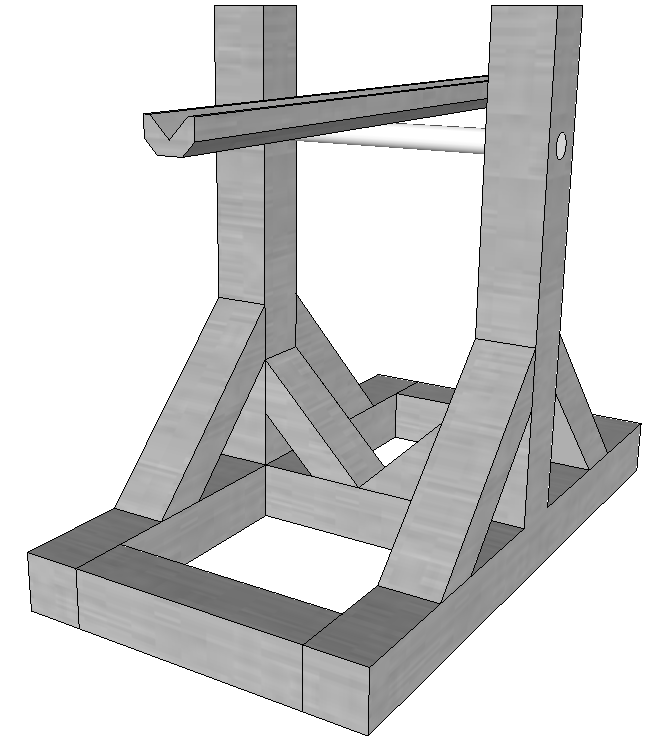
\includegraphics[width=0.4\textwidth]{cad}
	\caption{Render projektu CAD.}
	\label{fig:cad_render_1}
\end{figure}

Ostateczna konstrukcja różni się względem projektu \textsc{CAD} o wysokość słupów, i umiejscowienie łącznika między nimi. Dodatkowo zastosowano sztywne połączenie osi obrotu belki i samej belki wykorzystujące podpory wału.

%%%%%%%%
\section{Konstrukcja mechaniczna}

Większość konstrukcji powstała z ocynkowanych elementów stalowych, tzw. ,,ceowników'' w przekroju kwadratowym o boku długości \SI[mode=text]{4}{cm}, pozwalających na łatwe skręcanie kilku elementów ze sobą. Rozwiązanie to jest bardzo tanie w porównaniu do przemysłowych profili aluminiowych lub spawanych profili stalowych, ale jednocześnie jest dość ciężkie i poprzez niedomknięcie profilu podatne na pewne momenty gnące.

Kąty proste pomiędzy elementami ustawionymi prostopadle zostały zapewnione poprzez skręcenie za pomocą wsporników stalowych.

\begin{figure}[H]
	\centering
	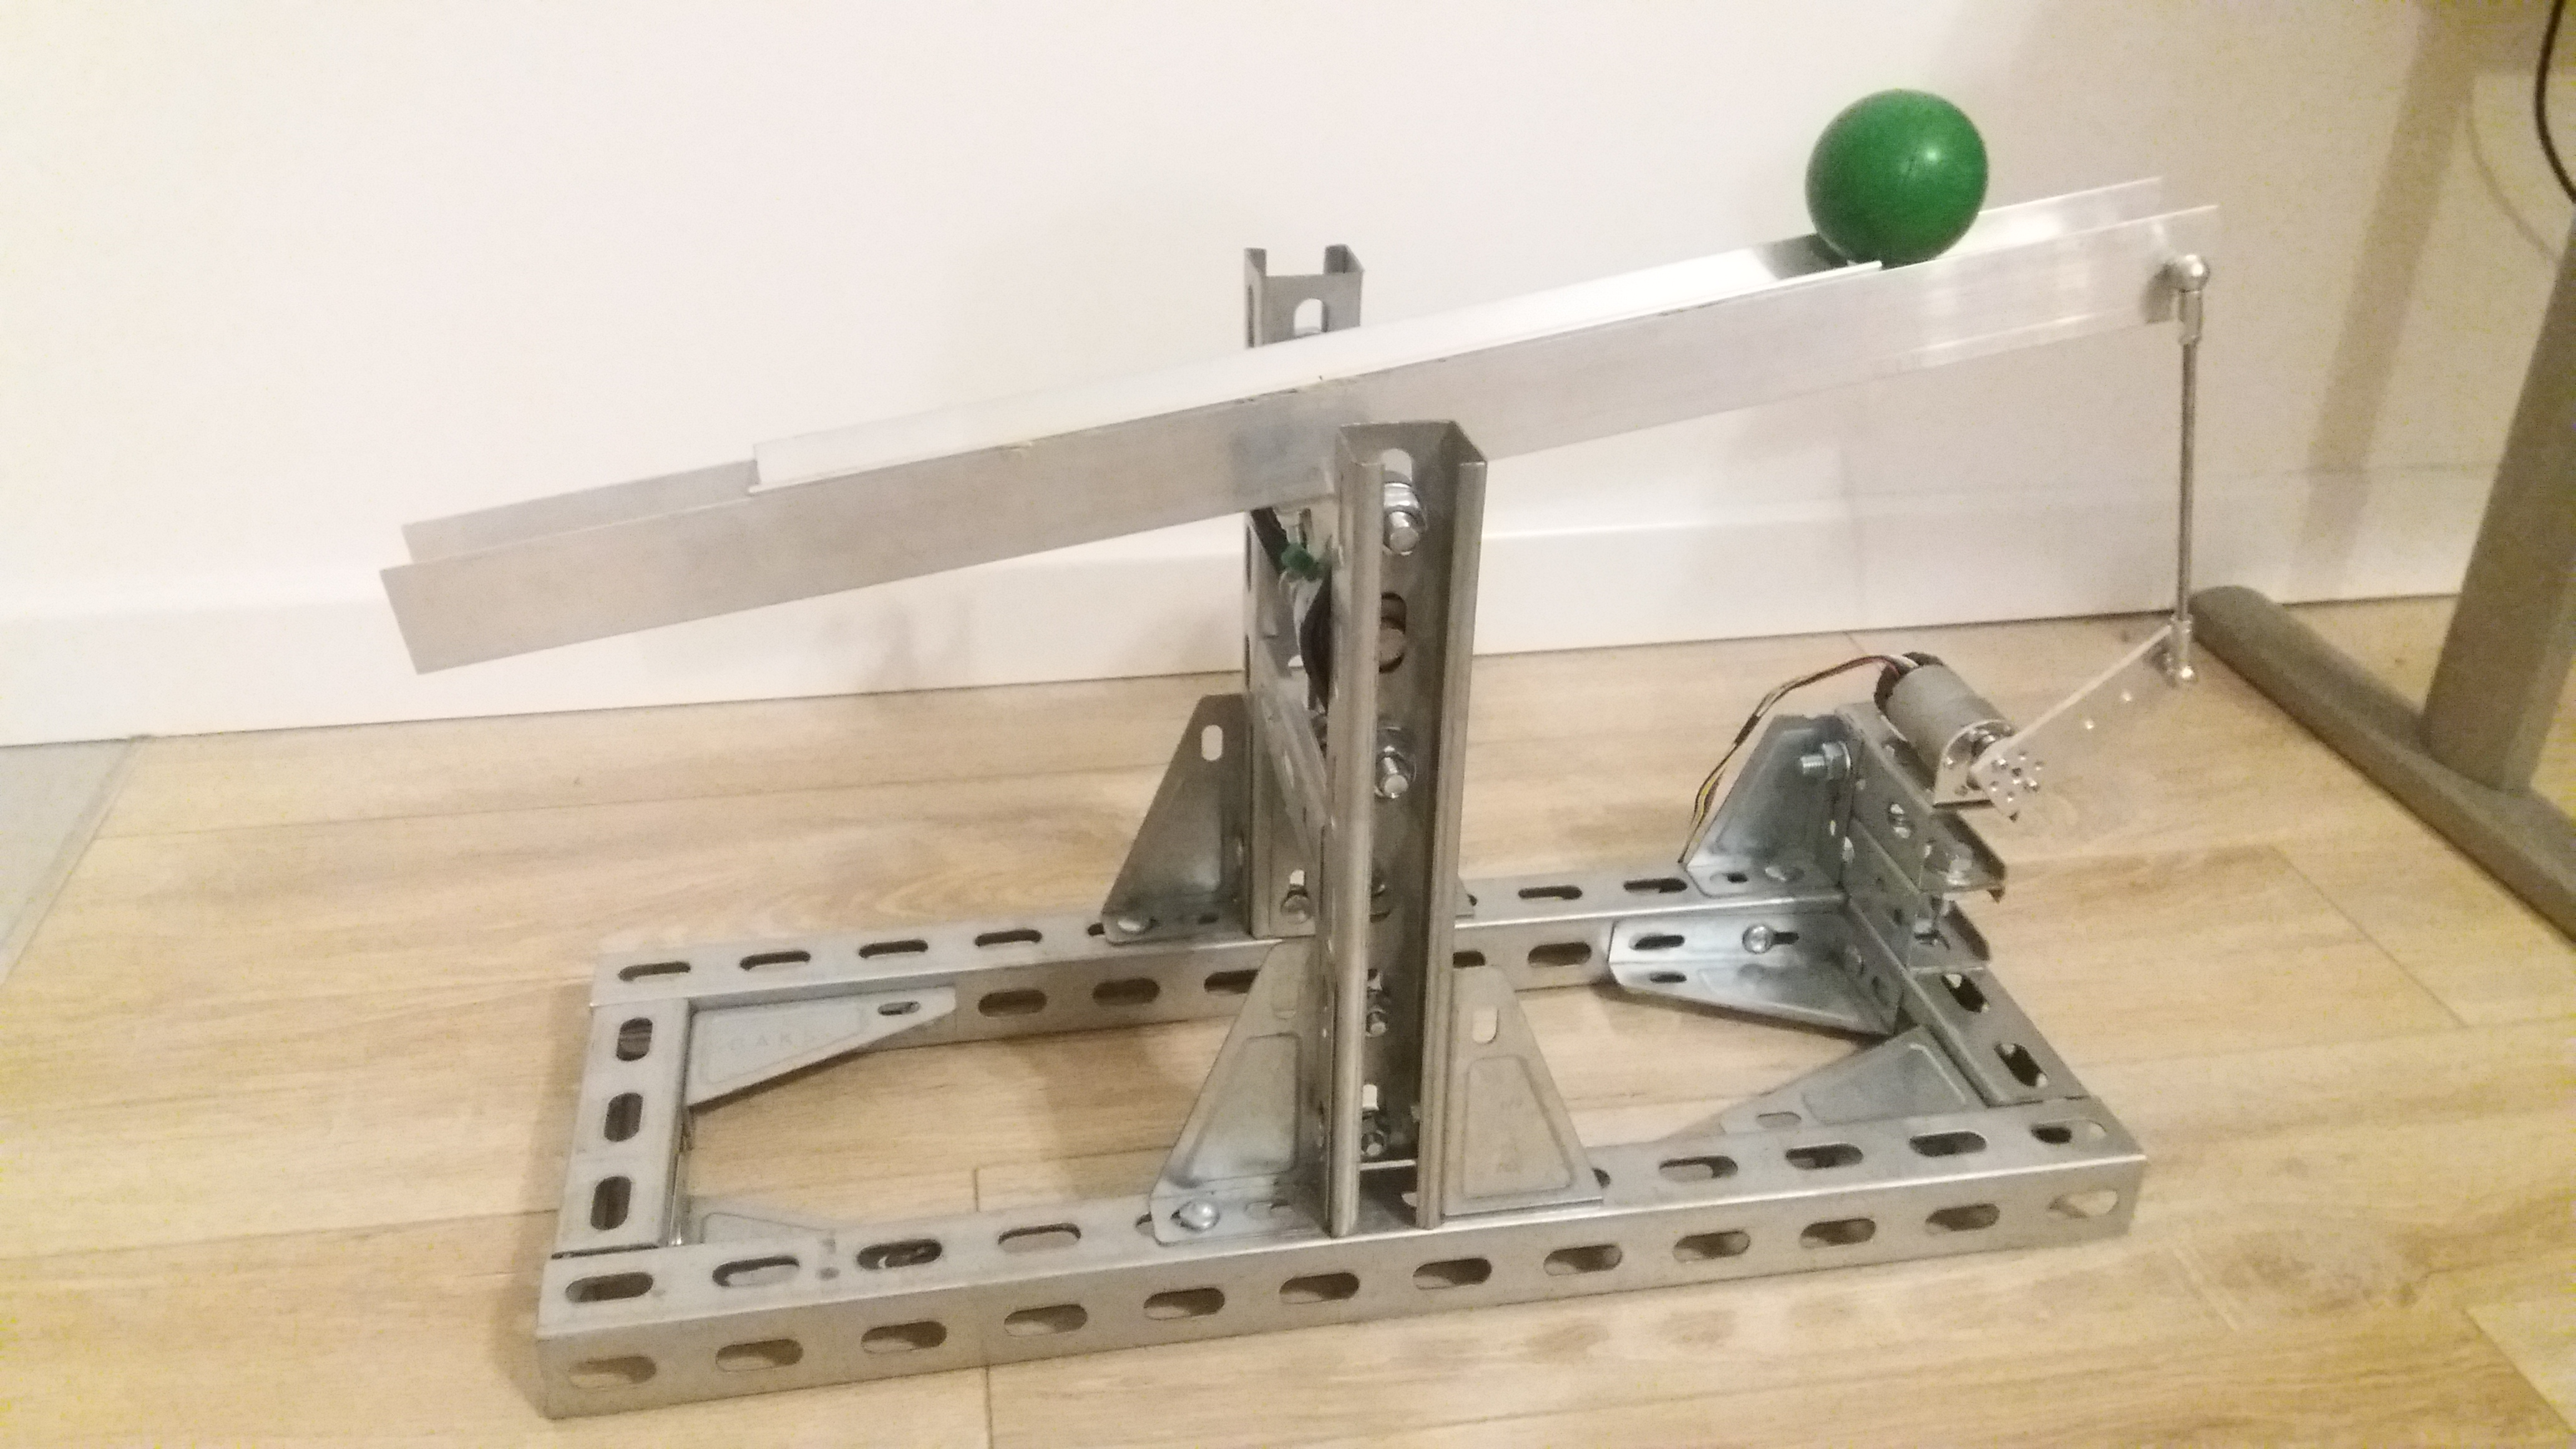
\includegraphics[width=0.7\textwidth]{mechatronics_perspective_1}
	\caption{Zdjęcie obiektu regulacji w trakcie budowy.}
	\label{fig:mechatronics_perspective_1}
\end{figure}

Na prostokątnej podstawie o wymiarach zewnętrznych \SI[mode=text]{60 x 23}{cm} wykonanej z ceowników ustawiono pionowo na środkach dłuższych boków słupy nośne, również wykonane z ceowników. Na słupach przyczepiono współosiowo łożyska maszynowe samonastawne typu UCFL 201 w obudowach odlewanych.

Słupy zostały usztywnione poprzez połączenie ich przęsłem podniesionym o \SI[mode=text]{11}{cm} względem podstawy.

Przez łożyska poprowadzono pręt nierdzewny stalowy o średnicy \SI[mode=text]{12}{mm}; na pręt nałożono podpory wałka w kształcie litery \texttt{T}, a do nich przykręcono belkę.

Silnik elektryczny, przymocowany do aluminiowego uchwytu, został umieszczony podłużnie na krótszym boku podstawy, na podwyższeniu wykonanym z dwóch elementów stalowych typu ceownik.

% TODO: podwyższenie zostało wzmocnione przeciwko gięciom poprzecznym i wzdłużnym poprzez zastosowanie …………

%%%%%%%%
\section{Przeniesienie napędu}

W obiekcie zastosowano przeniesienie napędu wykorzystujące mechanizm korbowy. Rozwiązanie to posiada kilka zalet:

\begin{itemize}
	\item gwarantuje bezpieczeństwo mechanizmu -- błąd algorytmiczny (np. przypadkowe podanie maksymalnego sterowania) nie spowoduje uszkodzenia fizycznego żadnej części obiektu,
	\item poprzez oddalenie punktu zaczepu korbowodu od osi obrotu belki zmniejsza wymagania dotyczące mocy silnika, a tym samym jego cenę,
	\item pozwala regulować zakres wychyleń belki w wyniku zmiany długości korby.
\end{itemize}

% TODO: napraw kolory w schemacie
% TODO: dodaj opis (korba, korbowód)
\begin{figure}[H]
	\centering
	\includesvg[width=0.6\textwidth,svgpath=./graphics/]{schemat_korba}
	\caption{Schemat napędu opartego o mechanizm korbowy.}
	\label{fig:schemat_korba}
\end{figure}

%%%%%%%%
\section{Belka}

Belka została stworzona poprzez trwałe sklejenie krawędzi kątownika aluminiowego o długości \SI[mode=text]{40}{cm} i boku \SI[mode=text]{3}{cm} oraz krawędzi ceownika aluminiowego o długości \SI[mode=text]{65}{cm} i boku \SI[mode=text]{4}{cm}. W przekroju przypomina to kształtem literę \texttt{M} domkniętą od spodu (\cref{fig:przekroj_belki}).

\begin{figure}[H]
	\centering
	\includesvg[width=0.2\textwidth,svgpath=./graphics/]{beam_xsection}
	\caption{Schemat przekroju belki z zaznaczonymi ceownikiem aluminiowym i kątownikiem aluminiowym.}
	\label{fig:przekroj_belki}
\end{figure}

Krótszy kątownik został umieszczony wzdłużnie na środku belki. W odległości około \SI[mode=text]{1}{cm} od jego końców zamontowano uchwyty na czujniki optyczne.

Uchwyty pozwalają na zmianę wysokości czujnika względem płaszczyzny belki, a także na pochylenie go w osi prostopadłej do płaszczyzny belki.

% TODO: schemat / render bracketu na czujnik

%%%%%%%%
\section{Kulka}

Do projektu dobrano lekką kulkę o masie \SI[mode=text]{20}{g} wykonaną z miękkiej gąbki; średnica kulki wynosi \SI[mode=text]{6}{cm}.

%---------------------------------------------------------------------------